\documentclass[aspectratio=169, table]{beamer}

\usepackage{listings}
\usepackage{tikz}
\usetikzlibrary{ fit, shapes.geometric, arrows.meta, positioning}
\usepackage{array}
\usepackage{float}
\usepackage{colortbl} 

\lstdefinestyle{RustStyle}{
	language=Java,
	morekeywords={println, Ok, async, fn, main, use, let, mut},
	basicstyle=\ttfamily\scriptsize,
	keywordstyle=\color{blue},
	commentstyle=\color{gray},
	stringstyle=\color{red},
	breaklines=true,
	showstringspaces=false,
	tabsize=2,
	captionpos=b,
	numbers=left,
	numberstyle=\tiny\color{gray},
	frame=lines,
	backgroundcolor=\color{lightgray!10},
	comment=[l]{//},
	morecomment=[s]{/*}{*/},
	commentstyle=\color{gray}\ttfamily,
	string=[s]{'}{'},
	morestring=[s]{"}{"},
	stringstyle=\color{teal}\ttfamily,
	%	showstringspaces=false
	literate=
	{\{}{{\textcolor{red}{\{}}}1
	{\}}{{\textcolor{red}{\}}}}1
	{:}{{\textcolor{red}{:}}}1
	{=}{{\textcolor{red}{=}}}1
	{.}{{\textcolor{red}{.}}}1
	{]}{{\textcolor{red}{]}}}1
	{[}{{\textcolor{red}{[}}}1
	{\#}{{\textcolor{red}{\#}}}1
	{;}{{\textcolor{red}{;}}}1
	{?}{{\textcolor{red}{?}}}1
	{!}{{\textcolor{red}{!}}}1
}

%\usepackage[beamertheme=./praditatheme]{Pradita}

\usetheme{Pradita}

\lstdefinelanguage{bash} {
	keywords={},
	basicstyle=\ttfamily\small,
	keywordstyle=\color{blue}\bfseries,
	ndkeywords={iex},
	ndkeywordstyle=\color{purple}\bfseries,
	sensitive=true,
	commentstyle=\color{gray},
	stringstyle=\color{red},
	numbers=left,
	numberstyle=\tiny\color{gray},
	breaklines=true,
	frame=lines,
	backgroundcolor=\color{lightgray!10},
	tabsize=2,
	comment=[l]{\#},
	morecomment=[s]{/*}{*/},
	commentstyle=\color{gray}\ttfamily,
	stringstyle=\color{purple}\ttfamily,
	showstringspaces=false
}


\title{\LARGE Orchestration-Driven\\Service-Oriented\\Architecture\\}
\subtitle{IF231303-Software Architecture}
\author{\textbf{Alfa Yohannis}}
\begin{document}
	
	\frame{\titlepage}
	
	
	\begin{frame}[fragile]
		\frametitle{Contents}
		\vspace{20pt}
		\begin{columns}[t]
			\column{0.5\textwidth}
			\tableofcontents[sections={1-5}]
			
			\column{0.5\textwidth}
			\tableofcontents[sections={6-10}]
		\end{columns}
	\end{frame}
	
\section{Pendahuluan}

\begin{frame}[fragile]{Pendahuluan: Orchestration-driven SOA}
	\vspace{10pt}
	\begin{columns}[T]
		\begin{column}{0.6\textwidth}
			\textbf{Definisi Umum}
			\begin{itemize}
				\item Orchestration-driven SOA = arsitektur layanan dengan komponen pusat: \textbf{orkestrator}.
				\item Orkestrator mengatur urutan eksekusi dan koordinasi layanan.
				\item Interaksi layanan dikendalikan berdasarkan workflow eksplisit.
			\end{itemize}
			
			\textbf{Karakteristik}
			\begin{itemize}
				\item Layanan bersifat loosely coupled dan reusable.
				\item Orkestrasi = \textbf{kontrol terpusat}, beda dari \textit{choreography} yang desentralisasi.
			\end{itemize}
		\end{column}
		
		\begin{column}{0.4\textwidth}
			\textbf{Konteks Penerapan}
			\begin{itemize}
				\item Digunakan dalam sistem enterprise dan integrasi antar aplikasi.
				\item Cocok untuk proses yang butuh:
				\begin{itemize}
					\item Konsistensi transaksi
					\item Pelacakan alur kerja
					\item Pengendalian proses kompleks
				\end{itemize}
				\item Didukung engine seperti Camunda, Zeebe, Temporal.
			\end{itemize}
		\end{column}
	\end{columns}
	\vspace{10pt}
\textit{Mendukung sistem modular, fleksibel, dan adaptif terhadap bisnis.}
\end{frame}


\section{Konsep Dasar}

\begin{frame}[fragile]{Konsep Dasar Orkestrasi Layanan}
	\vspace{20pt}
	\begin{columns}[T]
		\begin{column}{0.45\textwidth}
			\textbf{Apa itu Orchestration?} \\
			Orchestration adalah pengendalian urutan layanan oleh orchestrator. Ia mengeksekusi workflow, memanggil layanan, serta menangani input dan error. Pendekatan ini memberi kontrol dan visibilitas proses bisnis.
			
			\vspace{6pt}
			\textbf{Orchestration vs Choreography}
			\begin{itemize}
				\item \textbf{Orchestration}: kontrol terpusat.
				\item \textbf{Choreography}: interaksi antar layanan tanpa pusat.
			\end{itemize}
			
		\end{column}
		
		\begin{column}{0.55\textwidth}
			Orchestration cocok untuk proses kompleks; choreography lebih fleksibel dan ringan.
			
			\textbf{Komponen Orkestrasi}
			\begin{itemize}
				\item \textbf{Engine}: jalankan workflow (mis. Zeebe, Temporal).
				\item \textbf{Process}: urutan proses dalam BPMN/DSL.
				\item \textbf{Tasks}: panggil layanan eksternal.
				\item \textbf{Mapping}: konversi data antar langkah.
				\item \textbf{Monitoring}: pantau status dan log.
				\item \textbf{Error Handling}: retry, branching, kompensasi.
			\end{itemize}
		\end{column}
	\end{columns}
\end{frame}

\section{Contoh Kasus}
\begin{frame}[fragile]{Contoh Kasus Penggunaan ODSOA}
	\vspace{4pt}
	\begin{columns}[T]
		\begin{column}{0.5\textwidth}
			\textbf{1. Pemesanan Tiket Multi-Layanan} \\
			Orchestrator mengatur urutan layanan tiket, hotel, transportasi, dan pembayaran. Jika hotel penuh, orchestrator membatalkan pesanan lainnya. Proses jadi konsisten, otomatis, dan terdokumentasi.
			
			\vspace{6pt}
			\textbf{2. Automasi Proses Jasa} \\
			Pada klaim asuransi: formulir diproses, dokumen divalidasi OCR, data diverifikasi, kerusakan dihitung, klaim dibayar. Orkestrasi mempercepat dan mengurangi kerja berulang.
		\end{column}
		
		\begin{column}{0.5\textwidth}
			\textbf{3. Integrasi Aplikasi Enterprise} \\
			Saat onboarding:
			\begin{itemize}
				\item Tambah data di HR.
				\item Buat akun gaji.
				\item Alokasi anggaran awal.
				\item Notifikasi ke manajer.
			\end{itemize}
			Tanpa orkestrator, proses ini manual dan rawan kesalahan. Orkestrasi menjadikannya otomatis dan mudah diawasi.
		\end{column}
	\end{columns}
\end{frame}


\section{Kelebihan/Kekurangan}
\begin{frame}[fragile]{Kelebihan dan Kekurangan ODSA}
	\vspace{4pt}
	\begin{columns}[T]
		\begin{column}{0.5\textwidth}
			\textbf{Kelebihan}
			\begin{itemize}
				\item \textbf{Kontrol Terpusat:} Alur proses dikelola eksplisit dan mudah dipantau.
				\item \textbf{Fleksibel:} Logika proses bisa diubah tanpa menyentuh layanan.
				\item \textbf{Terukur:} Pengujian dan pemantauan proses lebih terstruktur.
				\item \textbf{Kolaboratif:} Tim bisnis buat workflow (BPMN), tim teknis fokus layanan.
			\end{itemize}
		\end{column}
		
		\begin{column}{0.5\textwidth}
			\textbf{Kekurangan}
			\begin{itemize}
				\item \textbf{Ketergantungan Orchestrator:} Titik rawan bottleneck jika tidak dirancang baik.
				\item \textbf{Debugging Lebih Sulit:} Perlu tracing dan logging yang kuat.
				\item \textbf{Overhead:} Manajemen status antar langkah menambah beban.
				\item \textbf{Tidak Efisien untuk Sederhana:} Untuk proses ringan, choreography bisa lebih cocok.
			\end{itemize}
		\end{column}
	\end{columns}
\end{frame}

\section{Arsitektur ODSOA}
\begin{frame}{Arsitektur Orchestration-driven SOA}
	\vspace{20pt}
	\centering
	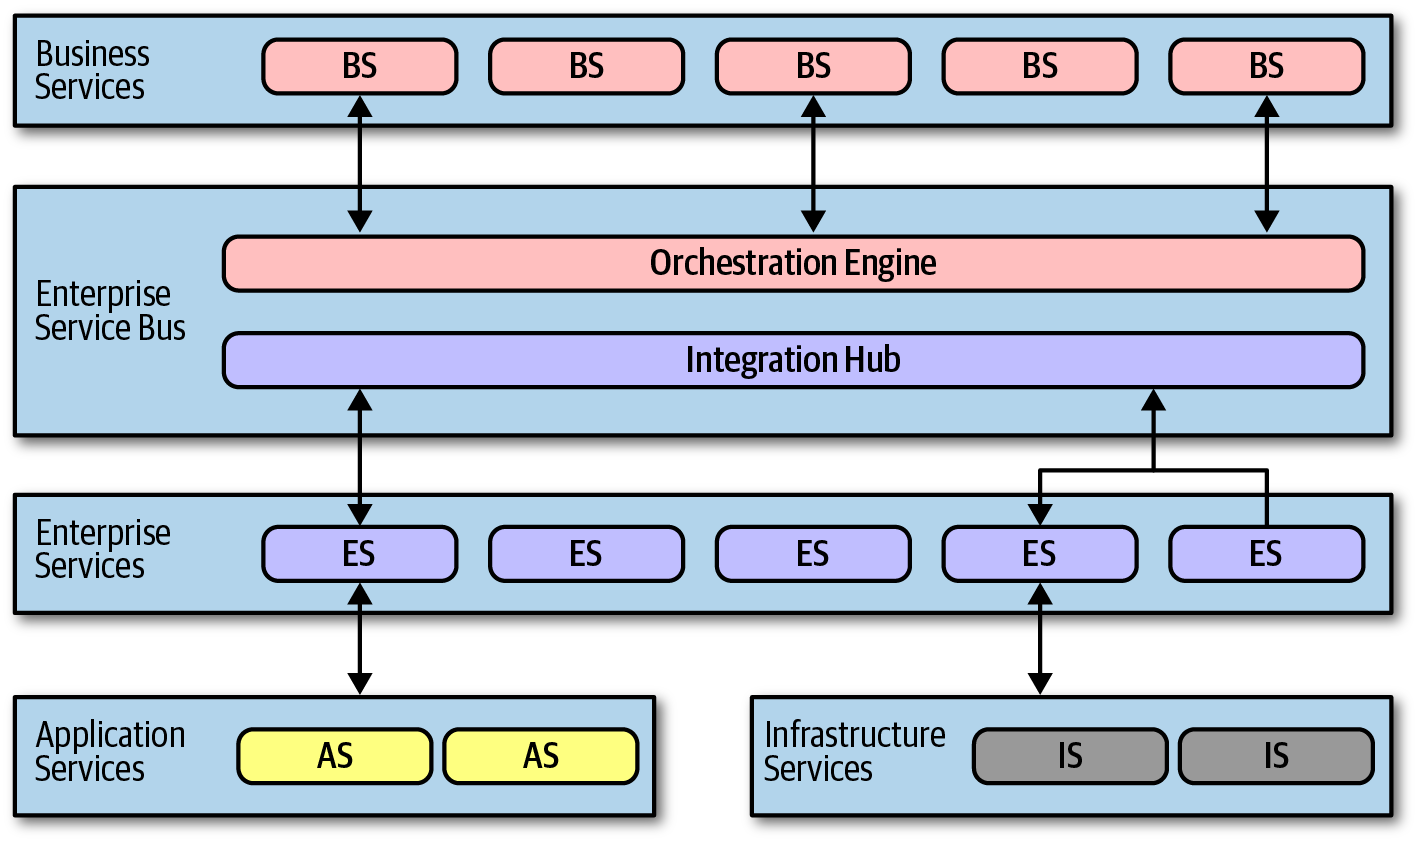
\includegraphics[width=0.8\textwidth]{../../images/orchestration-example}
\end{frame}

\begin{frame}[fragile]{Business \& Enterprise Services}
	\textbf{Business Services}:
	\begin{itemize}
		\item Mewakili logika proses tingkat tinggi: pemesanan, klaim, onboarding.
		\item Terdiri dari beberapa layanan lain dan dikendalikan via orchestrator.
		\item Contoh: \texttt{BookTravelPackage} memanggil layanan tiket, hotel, transportasi, pencatatan pelanggan via workflow BPMN (Camunda, Temporal).
	\end{itemize}
	
	\vspace{4pt}
	\textbf{Enterprise Services}:
	\begin{itemize}
		\item Layanan reusable dan atomik: \texttt{VerifyIdentity}, \texttt{CalculateScore}, \texttt{GenerateContract}.
		\item Menyatukan beberapa application services di bawahnya.
		\item Digunakan ulang dalam berbagai business service berbeda (pinjaman, rekening, kontrak vendor).
	\end{itemize}
\end{frame}

\begin{frame}[fragile]{ESB: Integration Hub}
	\textbf{Enterprise Service Bus (ESB)}:
	\begin{itemize}
		\item Middleware untuk pengiriman pesan, transformasi data (JSON/XML), routing, protokol.
		\item Umum: Apache ServiceMix, Mule ESB, Red Hat Fuse, WSO2.
		\item Peran modern digantikan oleh Kafka, service mesh, orchestrator event-driven.
	\end{itemize}
	
	\vspace{4pt}
	\textbf{Integration Hub}:
	\begin{itemize}
		\item Menyambungkan sistem berbeda (CRM, sistem lama, analitik).
		\item Fitur: normalisasi data, enrichment, routing, transformasi protokol.
		\item Teknologi: Apache Camel, Kafka Connect, Azure Logic Apps.
	\end{itemize}
\end{frame}

\begin{frame}[fragile]{ESB: Orchestration Engine}
	\textbf{Fungsi utama:}
	\begin{itemize}
		\item Menjalankan definisi proses (BPMN/DSL).
		\item Mengatur urutan eksekusi layanan, input/output, retry, dan kompensasi.
	\end{itemize}
	
	\vspace{4pt}
	\textbf{Contoh Engine:}
	\begin{itemize}
		\item \textbf{Camunda}: BPMN berbasis Java, cocok untuk enterprise.
		\item \textbf{Zeebe}: skalabel, event-driven, microservices.
		\item \textbf{Temporal}: pendekatan code-first, retry \& durabilitas terintegrasi.
	\end{itemize}
\end{frame}
\begin{frame}[fragile]{Application \& Infrastructure Services}
	\textbf{Application Services}:
	\begin{itemize}
		\item Menangani fungsi teknis spesifik: OCR, ML scoring, PDF generation.
		\item Biasanya terikat pada aplikasi tertentu.
		\item Contoh: \texttt{OCRApplicationService}, \texttt{MLScoringService}, \texttt{PDFGeneratorService}.
	\end{itemize}
	
	\vspace{4pt}
	\textbf{Infrastructure Services}:
	\begin{itemize}
		\item Menyediakan dukungan teknis dasar:
		\begin{itemize}
			\item Storage: PostgreSQL, MongoDB
			\item Messaging: Kafka, Redis
			\item Observability: Prometheus, Grafana, ELK
			\item Orkestrasi: Kubernetes
		\end{itemize}
		\item Termasuk service discovery (Consul) dan config management (Spring Cloud Config).
	\end{itemize}
\end{frame}

\section{Contoh: Pengajuan Pinjaman Digital}
\begin{frame}[fragile]{Contoh: Pengajuan Pinjaman Digital}
	Pengguna mengajukan pinjaman, lalu orchestrator menjalankan \texttt{LoanApplicationProcessing} sebagai business service. Langkahnya mencakup:
	\begin{itemize}
		\item \textbf{Enterprise Services:} \texttt{VerifyIdentity}, \texttt{EvaluateCreditworthiness}, \texttt{GenerateContract}
		\item \textbf{Application Services:} OCR dokumen, ML scoring, PDF generator
		\item \textbf{ESB:} menghubungkan Business Services dan Enterprise Services
		\item \textbf{Orchestrator:} Camunda atau Temporal mengelola eksekusi dan kompensasi
		\item \textbf{Integration Hub:} integrasi data CRM dan sistem lama
		\item \textbf{Infrastructure:} PostgreSQL, Redis, Kafka, Prometheus, Kubernetes
	\end{itemize}
\end{frame}

\section{Implementation Patterns}
\begin{frame}[fragile]{Pola Implementasi Orkestrasi}
	\vspace{20pt}
	\begin{columns}[T]
		\begin{column}{0.5\textwidth}
			\textbf{1. Centralized Orchestrator}
			\begin{itemize}
				\item Orchestrator pusat atur alur proses dan error handling.
				\item Layanan pasif, hanya merespons panggilan dari orchestrator.
				\item Contoh: alur order e-commerce. Tools: Camunda, Temporal.
			\end{itemize}
			
			\vspace{4pt}
			\textbf{2. Orchestrated Microservices}
			\begin{itemize}
				\item Satukan layanan kecil jadi workflow kompleks.
				\item Contoh: logistik $\rightarrow$ tracking $\rightarrow$ notifikasi.
				\item Butuh API jelas dan idempoten. Cocok untuk tim dan cloud-native.
			\end{itemize}
		\end{column}
		
		\begin{column}{0.5\textwidth}
			\textbf{3. Saga (Transaksi Panjang)}
			\begin{itemize}
				\item Setiap langkah punya kompensasi jika gagal.
				\item Cocok untuk transaksi multi-sistem, tanpa lock DB.
				\item Contoh: pembayaran $\rightarrow$ reservasi $\rightarrow$ rollback.
			\end{itemize}
			
			\vspace{4pt}
			\textbf{4. Monitoring dan Logging}
			\begin{itemize}
				\item Pantau status, error, dan audit proses.
				\item Gunakan correlation ID dan dashboard.
				\item Tools: Prometheus, Jaeger, ELK, Grafana.
			\end{itemize}
		\end{column}
	\end{columns}
\end{frame}

\section{Best Practices}
\begin{frame}[fragile]{Best Practices Orkestrasi Layanan}
	\vspace{10pt}
	\begin{columns}[T]
		\begin{column}{0.58\textwidth}
			\textbf{1. Kontrak Stabil} \\
			Gunakan kontrak API versi tetap (OpenAPI/gRPC). Hindari perubahan breaking, validasi input/output, dan sertakan definisi error yang jelas.
			
			\vspace{6pt}
			\textbf{2. Modular dan Reusable} \\
			Buat layanan tanggung jawab tunggal agar bisa digunakan lintas workflow. Modularitas memudahkan pengujian dan perawatan.
			
			\vspace{6pt}
			\textbf{3. Tangguh dan Tahan Error} \\
			Gunakan retry dengan backoff, fallback, dan kompensasi. Layanan harus idempoten. Aktifkan DLQ dan circuit breaker untuk stabilitas.
		\end{column}
		
		\begin{column}{0.42\textwidth}
			\textbf{4. Observabilitas dan Audit} \\
			Gunakan correlation ID untuk tracing. Integrasi observabilitas: Prometheus, Grafana, Jaeger, ELK/Loki.
			
			\vspace{6pt}
			Audit trail penting untuk debugging dan kepatuhan. Simpan histori proses secara aman dan terstruktur.
			
		\end{column}
	\end{columns}
\end{frame}

\section{Kesimpulan}
\begin{frame}[fragile]{Kesimpulan}
	\vspace{4pt}
	\begin{itemize}
		\item \textbf{Orchestration-driven SOA} mengelola proses bisnis kompleks melalui koordinasi layanan secara terpusat.
		\item Memungkinkan perancangan proses yang modular, terdokumentasi, dan mudah dimonitor.
		\item Cocok untuk integrasi antar sistem heterogen, termasuk legacy dan microservices.
		\item Kunci keberhasilan:
		\begin{itemize}
			\item Orchestrator andal (Camunda, Zeebe, Temporal)
			\item Kontrak API stabil dan terdokumentasi (OpenAPI, gRPC)
			\item Observabilitas menyeluruh (metrics, logs, tracing)
		\end{itemize}
		\item Tantangan: ketahanan sistem, desain kontrak, dan penanganan error.
		\item Dengan praktik terbaik, sistem menjadi adaptif, reusable, dan scalable untuk kebutuhan bisnis modern.
	\end{itemize}
\end{frame}


\end{document}
